\subsection{Sequential ABC: state of the art and limitations}
\label{sec:abc_smc}
Rejection-based ABC methods, including the enhanced permABC, remain computationally expensive due to their reliance on the prior as a proposal distribution. 
Most methods in the ABC literature rely instead on more sophisticated proposals. A typical strategy is to propose from some distribution \( q(\param) \), then assign importance weights  of the form \( \pi(\param)/q(\param) \) to accepted samples to correct for the fact that they are not drawn from the prior \( \pi(\cdot) \). This produces weighted samples from the ABC pseudo-posterior \( \pi_\varepsilon(\param \mid \obsdata) \). 

Sequential importance sampling further improves efficiency by constructing a sequence of proposal distributions \( q_t(\cdot) \) over \( T \) iterations. Inspired by the Sequential Monte Carlo (SMC) framework \citep{delmoralSequentialMonteCarlo2006a}, several ABC-SMC algorithms have been developed \citep{sisson2007sequential,sissonCorrectionSissonSequential2009, toniApproximateBayesianComputation2008, beaumontAdaptiveApproximateBayesian2009b, delmoralAdaptiveSequentialMonte2012}, significantly improving convergence and computational performance.

These methods differ in their algorithmic design but follow the same principle: simulate from a sequence of intermediate ABC pseudo-posteriors \( \pi_{\varepsilon_0}, \dots, \pi_{\varepsilon_T} \), where the thresholds satisfy \( \varepsilon_0 = \infty > \varepsilon_1 > \dots > \varepsilon_T = \varepsilon \). Weights are updated iteratively, enabling efficient progression from the prior \( \pi_{\varepsilon_0}(\cdot \mid \obsdata) = \pi(\cdot) \) to the target pseudo-posterior \( \pi_\varepsilon(\cdot \mid \obsdata) \).

Here, we adopt the algorithm proposed by \citet{delmoralAdaptiveSequentialMonte2012}, widely used as a benchmark for ABC methods \citep{clarte2021componentwise}. This method combines a random walk proposal (see Section~\ref{sec:kernels}) with a Metropolis–Rosenbluth-Teller-Hastings (MRTH) acceptance step based on the ABC criterion and the MRTH ratio. 
%
A notable feature of this algorithm is the possibility to simulate \( M \) datasets \( \simdata^{(1)}, \dots, \simdata^{(M)} \) per parameter value \( \param \). 
While increasing \( M \) can reduce variance in the acceptance decision, setting \( M = 1 \) leads to better computational efficiency, as shown in practice by \citet{delmoralAdaptiveSequentialMonte2012} and in theory by \citet{bornn2017use}. 
With $M=1$, the importance weights become binary: they are equal to 1 if the particle is accepted (i.e., the distance is below \( \varepsilon \)) and 0 otherwise.

This simplification, however, induces a limitation. When weights are binary, the Effective Sample Size (ESS) reduces to the number of surviving particles. While ESS is commonly used to assess sample quality, it may not accurately reflect the true diversity of the sample, especially when the acceptance threshold is low. In such scenarios, repeated resampling steps tend to concentrate the population, leading to particle degeneracy. 
To address this issue, we propose using the \emph{unique particle rate} as a complementary diagnostic. This metric, defined as the proportion of distinct parameter values among the accepted particles, provides a more sensitive indicator of sample diversity. It offers a practical way to monitor degeneracy and evaluate the effective exploration of the pseudo-posterior during the sequential process. 
In contrast, the ABC-PMC algorithm originally introduced by \citet{sissonCorrectionSissonSequential2009} and later corrected by \citet{beaumontAdaptiveApproximateBayesian2009b} uses multinomial resampling, a practice discouraged in the SMC literature due to its inefficiency \citep{chopin2020introduction}.

In the following subsections, we propose three ways to accelerate ABC-SMC with permutations, based on three different strategies to define intermediate distributions.

\subsection{The permABC-SMC algorithm}

The adaptive SMC algorithm proposed by \citet{delmoralAdaptiveSequentialMonte2012} can be seamlessly extended to the permABC framework. By substituting the standard ABC acceptance criterion with the permutation-based criterion \eqref{eqopti}, we develop a sequential algorithm that targets the pseudo-posterior distribution \( \tilde{\pi}_\varepsilon(\param \mid \obsdata) \).

Upon reaching the stopping criterion or when \( \varepsilon_T = \varepsilon \), we apply the projection step \eqref{eqproj} to each particle in the final population \( \{(\param^{T,i}, \simdata^{T,i})\}_{i=1}^N \). This yields samples from the permuted pseudo-posterior \( \pi_\varepsilon^*(\param \mid \obsdata) \), effectively restoring identifiability among compartments.

It is essential to ensure that the proposal distributions \( q_t(\cdot) \) are adapted to the new acceptance criterion. We detail such kernels in Section~\ref{sec:kernels}, emphasizing their role in maintaining the efficiency of the sampling process under the permutation-based framework.

This approach, termed \emph{permABC-SMC}, facilitates a sequential transition from the prior to the permuted pseudo-posterior \( \pi^*_\varepsilon(\param \mid \obsdata) \). Thanks to proposal kernels tailored to the permutation-based selection rule, permABC-SMC enhances the exploration of the parameter space, particularly in high-dimensional settings where standard ABC methods may struggle.

The permABC-SMC approach is a natural way to extend permABC into a sequential method. It relies on intermediate distributions of the form $(\pi^*_{\varepsilon_t})_t$ which are similar to Over-Sequential ABC methods, and it already leads to substantial computational gains, as shown in Section \ref{sec:numeric}. Before we examine these practical results, we introduce two innovative sequences of intermediate distributions, with novel selection criteria which are only available because we rely on permutation-based matching.

\subsection{Over-Sampling}
\label{sec:permABC_OS}
The Over-Sampling strategy leverages the flexibility of the permABC framework to sample more efficiently from the target pseudo-posterior \( \pi_\varepsilon^*(\cdot \mid \obsdata) \) by simulating more compartments than are present in the observed data. Specifically, instead of generating \( K \) pseudo-compartments, we simulate \( M > K \) compartments: that is, we consider \( \simdata \in \dataspace^M \) while the observed data remain in \( \dataspace^K \). We then accept or reject based on the best simulated subset of size $K$.

To implement this strategy, we draw \( \param = (\globparam, \locparam_1, \dots, \locparam_M) \sim \pi(\cdot) \), simulate the corresponding data \( \simdata = (z_1, \dots, z_M) \sim f(\cdot \mid \param) \), and use the following acceptance condition:
\begin{equation}
    \label{eq:os}
    \min_{\sigma \in \mathcal{A}_K^M} d(\obsdata, \simdata_{\sigma}) \leq \varepsilon,
\end{equation}
where \( \mathcal{A}_K^M \) denotes the set of injections from \( \{1, \dots, K\} \) to \( \{1, \dots, M\} \), i.e., the set of partial \( K \)-permutations of \( \{1, \dots, M\} \). As in \eqref{eqopti}, this optimization problem can be solved efficiently using the same assignment algorithm with computational complexity \( \mathcal{O}(K^2 M) \) \citep{crouseImplementing2DRectangular2016a}.

We slightly abuse notation by denoting \( f \) the joint simulator over compartments, regardless of whether the number of compartments is \( K \) (observed) or \( M \) (simulated). This is justified since the simulator is defined componentwise via a common mechanism \( g \), applied independently to each compartment: formally, \( f(\simdata \mid \param) := \prod_{m=1}^M g(z_m \mid \globparam, \locparam_m) \).
 
Analogously to the case \( M = K \), this procedure defines a pseudo-posterior distribution \( \tilde{\pi}_\varepsilon^M(\cdot \mid \obsdata) \), and its projected version \( \pi_\varepsilon^{*M}(\cdot \mid \obsdata) \), which is obtained by applying the optimal partial permutation minimizing \eqref{eq:os} in a reasoning analogous to that of Section~\ref{secabc_to_permabc} (see Appendix~\ref{appendix_os} for details).

\new{More precisely, Over-Sampling can be viewed as a pushforward construction. Let \( \sigma^*=\sigma^*(\param,\simdata,\obsdata) \in \arg\min_{\sigma \in \mathcal{A}_K^M} d(\obsdata,\simdata_\sigma) \), using any measurable tie-breaking rule, and define the matching map}
\begin{equation}
    \Psi_{\obsdata}^{(M)} : (\param,\simdata) \longmapsto (\param^*,\simdata^*),
\end{equation}
\new{where}
\begin{equation}
    \simdata^* = \simdata_{\sigma^*} \in \dataspace^K,
    \qquad
    \param^* = \bigl(\globparam,\locparam_{\sigma^*(1)},\dots,\locparam_{\sigma^*(K)}\bigr).
\end{equation}
\new{Then the projected Over-Sampling distribution is exactly the pushforward}
\begin{equation}
    \pi_\varepsilon^{*M}(\cdot \mid \obsdata)
    =
    \bigl(\Psi_{\obsdata}^{(M)}\bigr)_\#
    \tilde{\pi}_\varepsilon^M(\cdot \mid \obsdata).
\end{equation}
\new{In other words, \( \tilde{\pi}_\varepsilon^M \) is the ABC law on the enlarged space \( (\globparam,\locparam_{1:M},\simdata_{1:M}) \), while \( \pi_\varepsilon^{*M} \) is obtained by projecting onto the \(K\) matched compartments and their associated local parameters.}

\old{Interestingly, the marginals in $\globparam$ and $\locparam$ exhibit contrasting behaviors as $M$ varies. When $M$ is large, the acceptance condition becomes easier to satisfy regardless of the value of $\varepsilon$, leading to a joint pseudo-posterior distribution close to the prior. Since the permutation only affects the local parameters, the marginal over $\globparam$ remains nearly unchanged, and therefore close to its prior distribution. In contrast, the marginal over the local parameters becomes more concentrated. This is because, when $M$ is large, the optimization in \eqref{eq:os} explores a wider set of potential matches, and the local parameters $\locparam_{1:K}$ corresponding to the best matching compartments are those that generate data most similar to $\obsdata$ under a given $\globparam$. As a result, these local components become tightly clustered around values that are locally optimal with respect to the matching criterion. As $M$ decreases toward $K$, this concentration fades, and the marginal over $\locparam$ gradually approaches the full permABC pseudo-posterior. This behavior is illustrated in Figure~\ref{fig:os}, and further discussed in Appendix~\ref{appendix_os}.}

\new{This pushforward representation also yields a clean asymptotic description of the regime \( M \to \infty \). Define}
\begin{equation}
    d_M(\obsdata,\simdata_{1:M})
    :=
    \min_{\sigma \in \mathcal{A}_K^M} d(\obsdata,\simdata_\sigma),
\end{equation}
\new{and, for fixed \( \globparam \), let}
\begin{equation}
    g_{\globparam}(z)
    :=
    \int g(z \mid \globparam,\mu)\,\pi(d\mu),
    \qquad
    S_{\globparam}
    :=
    \operatorname{supp}(g_{\globparam}).
\end{equation}
\new{We then introduce the support-based discrepancy}
\begin{equation}
    \delta_{\globparam}(\obsdata)
    :=
    \inf_{x_{1:K}\in S_{\globparam}^K} d(\obsdata,x_{1:K}).
\end{equation}
\new{Under mild regularity assumptions on \( d \), if \( Z_1,\dots,Z_M \mid \globparam \stackrel{\text{i.i.d.}}{\sim} g_{\globparam} \), then}
\begin{equation}
    d_M(\obsdata,Z_{1:M})
    \xrightarrow[M\to\infty]{a.s.}
    \delta_{\globparam}(\obsdata).
\end{equation}
\new{Hence, for every \( \varepsilon \) away from the boundary case \( \delta_{\globparam}(\obsdata)=\varepsilon \),}
\begin{equation}
    \mathbb{P}_{\globparam}\!\Bigl(
        d_M(\obsdata,Z_{1:M}) \le \varepsilon
    \Bigr)
    \xrightarrow[M\to\infty]{}
    \mathbf{1}\!\left\{
        \delta_{\globparam}(\obsdata)\le \varepsilon
    \right\}.
\end{equation}
\new{Therefore the marginal Over-Sampling pseudo-posterior on the global parameter satisfies}
\begin{equation}
    \tilde{\pi}_\varepsilon^M(\globparam \mid \obsdata)
    \propto
    \pi(\globparam)\,
    \mathbb{P}_{\globparam}\!\Bigl(
        d_M(\obsdata,Z_{1:M}) \le \varepsilon
    \Bigr)
    \xrightarrow[M\to\infty]{}
    \pi(\globparam)\,
    \mathbf{1}\!\left\{
        \delta_{\globparam}(\obsdata)\le \varepsilon
    \right\}.
\end{equation}
\new{In particular, if \( \delta_{\globparam}(\obsdata)=0 \) for every \( \globparam \) in the support of the prior, then for every \( \varepsilon>0 \),}
\begin{equation}
    \tilde{\pi}_\varepsilon^M(\globparam \mid \obsdata)
    \xrightarrow[M\to\infty]{}
    \pi(\globparam).
\end{equation}
\new{Thus, infinite Over-Sampling destroys all information on the global parameter: asymptotically, the ABC acceptance event no longer measures whether \( \globparam \) reproduces the observed compartments with the correct probability, but only whether the observed data lie in the support of the local marginal model. By contrast, the pushforward map \( \Psi_{\obsdata}^{(M)} \) still retains the \(K\) matched local parameters \( \locparam_{\sigma^*(1:K)} \), which explains why local marginals may become concentrated around good matching values even when the marginal in \( \globparam \) becomes nearly flat. As \( M \) decreases back to \( K \), this degeneracy disappears and the family \( \pi_\varepsilon^{*M} \) connects back continuously to the standard permABC pseudo-posterior. This behavior is illustrated in Figure~\ref{fig:os}, and further discussed in Appendix~\ref{appendix_os}.}

This new distribution family is particularly appealing, as it introduces a natural sequence of auxiliary distributions that converge to the target distribution \( \pi_\varepsilon^*(\cdot \mid \obsdata) \). We define a decreasing sequence \( M_0 > M_1 > \cdots > M_T = K \), keeping \( \varepsilon \) fixed, such that the acceptance condition \eqref{eq:os} becomes increasingly selective until it recovers the standard permABC criterion \eqref{eqopti} when \( M = K \). 
To navigate this sequence \( \left \{\tilde{\pi}_\varepsilon^{M_t}, t = 0, \dots, T \right\} \), we adapt the ABC-SMC framework of \citet{delmoralAdaptiveSequentialMonte2012}, as discussed in Section~\ref{sec:abc_smc}. At each stage, we apply the optimal partial permutation \( \sigma^* \) to each accepted particle to obtain a sample from \( \pi_\varepsilon^*(\cdot \mid \obsdata) \). This results in a new algorithm we call \emph{permABC-Over-Sampling (permABC-OS)}.

This method allows convergence to the target distribution in a reduced number of iterations. However, it also introduces several challenges that we now discuss. The first requirement for the success of the method is to initialize the algorithm with a sufficiently large and diverse population of accepted particles. To achieve this, one must choose $M_0$ and $\varepsilon$ in a coordinated manner. Specifically, since the minimum in \eqref{eq:os} decreases with $M$, a smaller value of $\varepsilon$ necessitates a larger $M_0$ in order to maintain a reasonable acceptance rate at the first iteration. In Appendix~\ref{appendix_os}, we propose a method to calibrate $\varepsilon$ as a function of $M_0$, thereby allowing users to set $M_0$ under a fixed simulation budget.

A second challenge attached to this method is the risk of extinction of the particle population during the sequential iterations. Specifically, when transitioning from population $t$ with $M_t$ compartments to population $t+1$ with $M_{t+1} < M_t$, the acceptance condition \eqref{eq:os} is evaluated on a reduced subset of simulated compartments. If compartments that previously matched observed ones are no longer considered, the particle may be rejected—even though it was previously accepted. To mitigate this, the sequence $M_t$ must be selected carefully. We provide a practical heuristic for this in Appendix~\ref{appendix_os}. 

Even under a careful design of the sequence $M_t$, a large portion of the population may be lost in this transition. To address this issue, we introduce a duplication mechanism whereby each particle is replicated across multiple random permutations. This increases the probability that at least one version of the particle survives the next acceptance test, without requiring additional simulations. The duplication strategy, along with heuristic guidelines for both selecting the sequence \( (M_t) \) and tuning \( \varepsilon \), is also detailed in Appendix~\ref{appendix_os}. 

\begin{figure}[htbp]
    \centering
    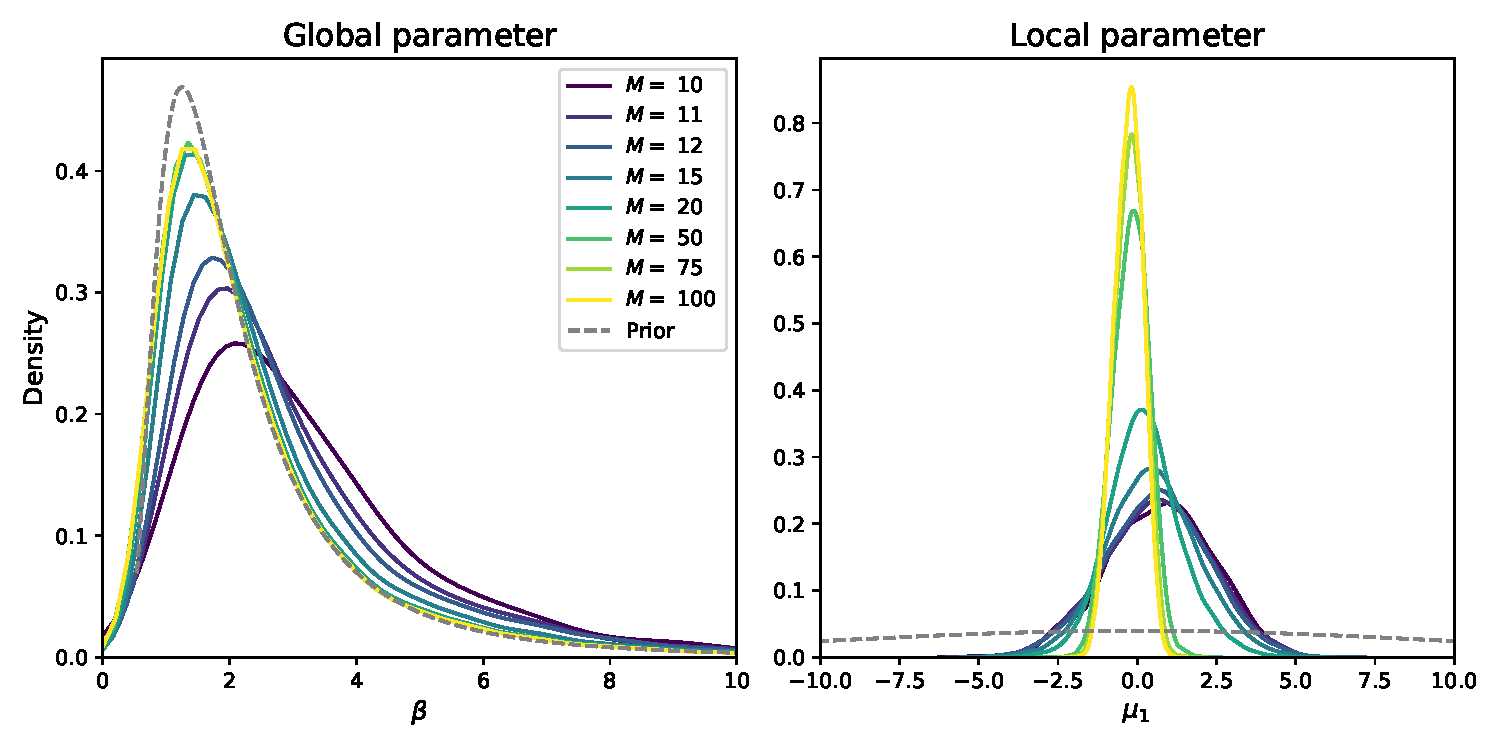
\includegraphics[scale=.5]{fig/fig2.pdf}
    \caption{Evolution of the pseudo-posterior \( \pi_\varepsilon^{*M} \) as \( M \) decreases from \( M_0 = 150 \) (yellow) to \( M_T = K = 10 \) (purple) for a Gaussian toy model.}
    \label{fig:os}
\end{figure}


\subsection{Under-Matching}
\label{sec:undermatching}
The under matching strategy—referred to as \emph{permABC-Under-Matching (permABC-UM)}—adopts a  perspective opposite to Over-Sampling. 
In this approach, we simulate synthetic data with the same number $K$ of compartments as the observed data; but at intermediate steps, we no longer require the simulated data to match all $K$ observed compartments. Instead, we simulate $K$ compartments but only require $L<K$ to match. The resulting acceptance criterion is defined as:
\begin{equation}
    \label{eqopti_um}
    \min_{\sigma \in \mathcal{A}_L^{K}, \tilde{\sigma} \in \mathcal{A}_L^{K}} d(\obsdata_{\tilde \sigma}, \simdata_{\sigma}) \leq \varepsilon,
\end{equation}
where \( \sigma \) and \( \tilde{\sigma} \) denote the sets of \( L \) selected compartments from the simulated and observed datasets, respectively. 


To solve this optimization problem efficiently, we extend the cost matrix by adding \( K - L \) dummy rows and \( K - L \) dummy columns with zero cost. These artificial entries ensure that \( K - L \) assignments are trivially matched, leaving the algorithm to find the best \( L \) true matches. This reduces the partial matching problem to a standard linear sum assignment problem on a square matrix of size \( (2K - L) \times (2K - L) \), which can be solved in \( \mathcal{O}\{(2K-L)^3\} \) time using classical algorithms \citep{crouseImplementing2DRectangular2016a}. 
 

This formulation allows for the algorithm to search over all possible \( L \)-sized subsets in both datasets, thereby relaxing the matching constraint and increasing flexibility in early iterations.

Although the distance \( d \) in Equation~\eqref{eqdistance} is defined for full datasets in \( \dataspace^K \), it naturally extends to subsets. In this context, given \( \sigma, \tilde \sigma \in \mathcal{A}_L^K \), the restricted distance is such that
\[
d(\obsdata_{\tilde \sigma}, \simdata_{\sigma})^2 = {\sum_{k=1}^L w_{\tilde \sigma(k)}^2 \| \obsdata_{\tilde \sigma(k)} - \simdata_{\sigma(k)} \|_2^2}.
\]
This formulation implies that compartments with higher weights have a greater impact on the acceptance condition, and are thus harder to match. This property can be exploited to prioritize compartments deemed more informative or robust, by appropriately adjusting the weights \( w_k \).

As in other variants of permABC, we employ a SMC scheme through a sequence of intermediate distributions \( \tilde{\pi}_\varepsilon^{L_t} \), corresponding to an increasing schedule \( L_0 < L_1 < \dots < L_T = K \). This gradual tightening of the matching criterion provides a smooth path toward the final target \( \pi^*_\varepsilon(\cdot \mid \obsdata) \), where all compartments are required to match.

Nevertheless, permABC-Under-Matching faces challenges similar to those of the Over-Sampling approach. In particular, it is crucial to select the initial tolerance \( \varepsilon \) appropriately, so as to ensure a sufficiently large and diverse first population. This requires calibrating \( \varepsilon \) as a function of \( L_0 \), the initial number of matched compartments, towards guaranteeing a high survival rate at the start of the algorithm.

Moreover, when the model is misspecified for even a single observed compartment, the final transition from \( L_{T-1} = K - 1 \) to \( L_T = K \) can lead to a sharp drop in the acceptance rate, resulting in severe particle degeneracy or even extinction. This makes the design of the sequence \( (L_t) \) and the level \( \varepsilon \) particularly critical for the success of the method. 
We show in Section \ref{sec:osum} that a well-designed under matching approach can increase performance in the presence of outliers.

These aspects are discussed in Appendix~\ref{appendix_um}, along with practical guidelines for choosing \( L_t \) and calibrating \( \varepsilon \) to avoid degeneracy. Situations where permABC-Under-Matching is especially advantageous, such as in the presence of outliers or structural model misspecification, are further investigated in Section~\ref{sec:osum}.

\subsection{Proposal Kernels for Permuted Inference}
\label{sec:kernels}


We recall that, by the abuse of notation introduced previously, we write \( \param_\sigma = (\globparam, \locparam_{\sigma(1)}, \dots, \locparam_{\sigma(K)}) \) to denote the parameter vector permuted by a given \( \sigma \in \mathcal{S}_K \), acting on the local components.


In the ABC-SMC framework of \citet{delmoralAdaptiveSequentialMonte2012}, the MCMC kernel \( K_t \) at iteration \( t \) uses a Gaussian random walk proposal \( q_t \) of the form:
\[
q_t(\cdot \mid \param) = \mathcal{N}\bigl\{\param, \operatorname{diag}\bigl(\tau_t^2\bigr)\bigr\},
\]
where \( \tau_t^2 \in \mathbb{R}^d \) is a vector of componentwise variances. These are typically defined as:
\[
\tau_t^2 = 2 \cdot \operatorname{var}\bigl\{\bigl(\param^{t-1,i}\bigr)_i\bigr\},
\]
i.e., twice the empirical variance across particles from the previous population. A Metropolis–Hastings correction step is then applied using the ABC acceptance criterion.

In the case of permABC-SMC, the exchangeability of the local parameters introduces label switching in the particle populations, which complicates the direct computation of componentwise variances. To resolve this, we first align the local parameters across particles using their optimal permutations \( \sigma_i^* \), and compute:
\[
\tau_t^2 = 2 \cdot \operatorname{var}\bigl\{\bigl(\param_{\sigma_i^*}^{t-1,i}\bigr)_i\bigr\}.
\]
This alignment restores parameter consistency across compartments, and allows us to maintain a diagonal Gaussian kernel with meaningful componentwise variances. The proposal kernel is then given by:
\[
q_t(\cdot \mid \param, \sigma) = \mathcal{N}\bigl[\param, \operatorname{diag}\bigl\{\sigma^{-1}(\tau_t^2)\bigr\}\bigr],
\]
where \( \sigma^{-1}(\tau_t^2) \) permutes the variance vector accordingly, so that each coordinate of \( \param \) is perturbed using the variance estimated in the appropriate reference frame.

In the case of \emph{Over-Sampling}, when the number of simulated compartments \( M \) exceeds the number of observed compartments \( K \), only a subset of the local parameters are matched to observations at each iteration. Let \( \mathcal{I} = \mathrm{Im}(\sigma^*) \subset \{1, \dots, M\} \) denote the indices of simulated compartments that are matched. For those indices, we reuse the corresponding variances from \( \tau_t^2 \) defined above. For the unmatched components \( k \notin \mathcal{I} \), we assign a default value:
\[
\tau_0^2 := \max_{k \in \mathcal{I}} \tau_t^2[k],
\]
which ensures exploration and numerical stability. This same default value \( \tau_0^2 \) is reused in the under-matching case below.





In the case of \emph{Under-Matching}, only a subset \( L_t < K \) of the observed compartments is matched at each iteration. For each particle \( i \), we define two injective mappings: \( \sigma_i \in \mathcal{A}_L^K \), which maps observed compartments to simulated compartments and \( \tilde{\sigma}_i \in \mathcal{A}_L^K \), which maps simulated compartments to observed ones.

The composition \( \tilde{\sigma}_i^{-1} \circ \sigma_i \) defines a partial permutation over observed indices, recovering the correspondence between an observed compartment \( k \in \{1, \dots, K\} \) and its matched simulated counterpart (when such a match exists for particle \( i \)). This matching allows us to construct a permutation-adjusted empirical variance over the population:
\[
\tau_t^2[k] = 2 \cdot \operatorname{Var} \left\{ \theta^{t-1,i}_{\tilde{\sigma}_i^{-1} \circ \sigma_i(k)} \right\}_i,
\]
defined only for those \( k \) that are matched in a sufficient number of particles. For unmatched coordinates, a default prior variance \( \tau_0^2 \) is used.


% In the case of under matching, only a subset \( L_t < K \) of observed compartments are matched at each iteration. Let \( \sigma \in \mathcal{A}_L^K \) and \( \tilde \sigma \in \mathcal{A}_L^K \) be the injections representing matches from observed to simulated compartments and vice versa. For each observed coordinate \( k \in \{1,\dots,K\} \), we define:
% \[
% \tau_t^2[k] = 2 \cdot \operatorname{var}\bigl\{\bigl(\theta_{\tilde \sigma_i^{-1} \circ \sigma_i(k)}^{t-1,i}\bigr)_i\bigr\},
% \]
% whenever the compartment \( k \) has been matched frequently enough across the population. If this condition is not met (e.g., in early iterations or due to sparse matching), we fallback to the default value \( \tau_t^2[k] = \tau_0^2 \).

% These variance assignment strategies allow us to construct robust and coherent Gaussian random walk proposals \( q_t \) for both global and local parameters across all three regimes: permABC-SMC, Over-Sampling, and Under-Matching.


These strategies ensure that Gaussian random walk proposals remain coherent and effective across all three regimes — standard permABC, Over-Sampling, and Under-Matching — by providing consistent scaling for both global and local parameters.

